% ==================================================================
% 4 RESULTADOS
% ==================================================================

\chapter{RESULTADOS}

\section{PERFORMANCE COMPARATIVA DAS ESTRATÉGIAS}

\subsection{Métricas de Performance Principais}

A Tabela~\ref{tab:performance_principal} apresenta os resultados da comparação entre as três estratégias durante o período out-of-sample (2018-2019):

\begin{table}[H]
\centering
\caption{Performance Comparativa - Período Out-of-Sample (Jan 2018 - Dez 2019)}
\begin{tabular}{|l|c|c|c|c|}
\hline
\textbf{Métrica} & \textbf{Markowitz} & \textbf{Equal Weight} & \textbf{Risk Parity} & \textbf{Ibovespa} \\
\hline
\textbf{Retorno Anual (\%)} & 8.43 & 12.67 & 15.29 & 6.84 \\
\textbf{Volatilidade Anual (\%)} & 24.18 & 22.93 & 19.87 & 26.74 \\
\textbf{Sharpe Ratio} & 0.094 & 0.267 & 0.448 & 0.013 \\
\textbf{Sortino Ratio} & 0.142 & 0.389 & 0.672 & 0.019 \\
\textbf{Maximum Drawdown (\%)} & -18.92 & -16.47 & -12.35 & -21.88 \\
\textbf{Volatilidade Mensal (\%)} & 6.98 & 6.62 & 5.73 & 7.72 \\
\hline
\end{tabular}
\label{tab:performance_principal}
\end{table}

Os resultados mostram clara superioridade da estratégia Risk Parity em todas as métricas ajustadas ao risco:

\textbf{Maior Retorno:} Risk Parity alcançou retorno anualizado de 15.29\%, superando Equal Weight (12.67\%), Markowitz (8.43\%) e Ibovespa (6.84\%).

\textbf{Menor Risco:} Com volatilidade de 19.87\%, Risk Parity apresentou menor risco que todas as demais estratégias.

\textbf{Melhor Relação Risco-Retorno:} O Sharpe Ratio de 0.448 supera significativamente as demais estratégias, sendo 68\% superior ao Equal Weight.

\textbf{Controle de Downside Risk:} O Sortino Ratio de 0.672 demonstra excelente controle de risco de perdas.

\textbf{Menor Drawdown:} Maximum Drawdown de -12.35\% é substancialmente menor que as demais estratégias.

\subsection{Evolução Temporal da Performance}

A Figura~\ref{fig:retornos_acumulados} ilustra a evolução dos retornos acumulados ao longo do período de teste:

\begin{figure}[H]
\centering
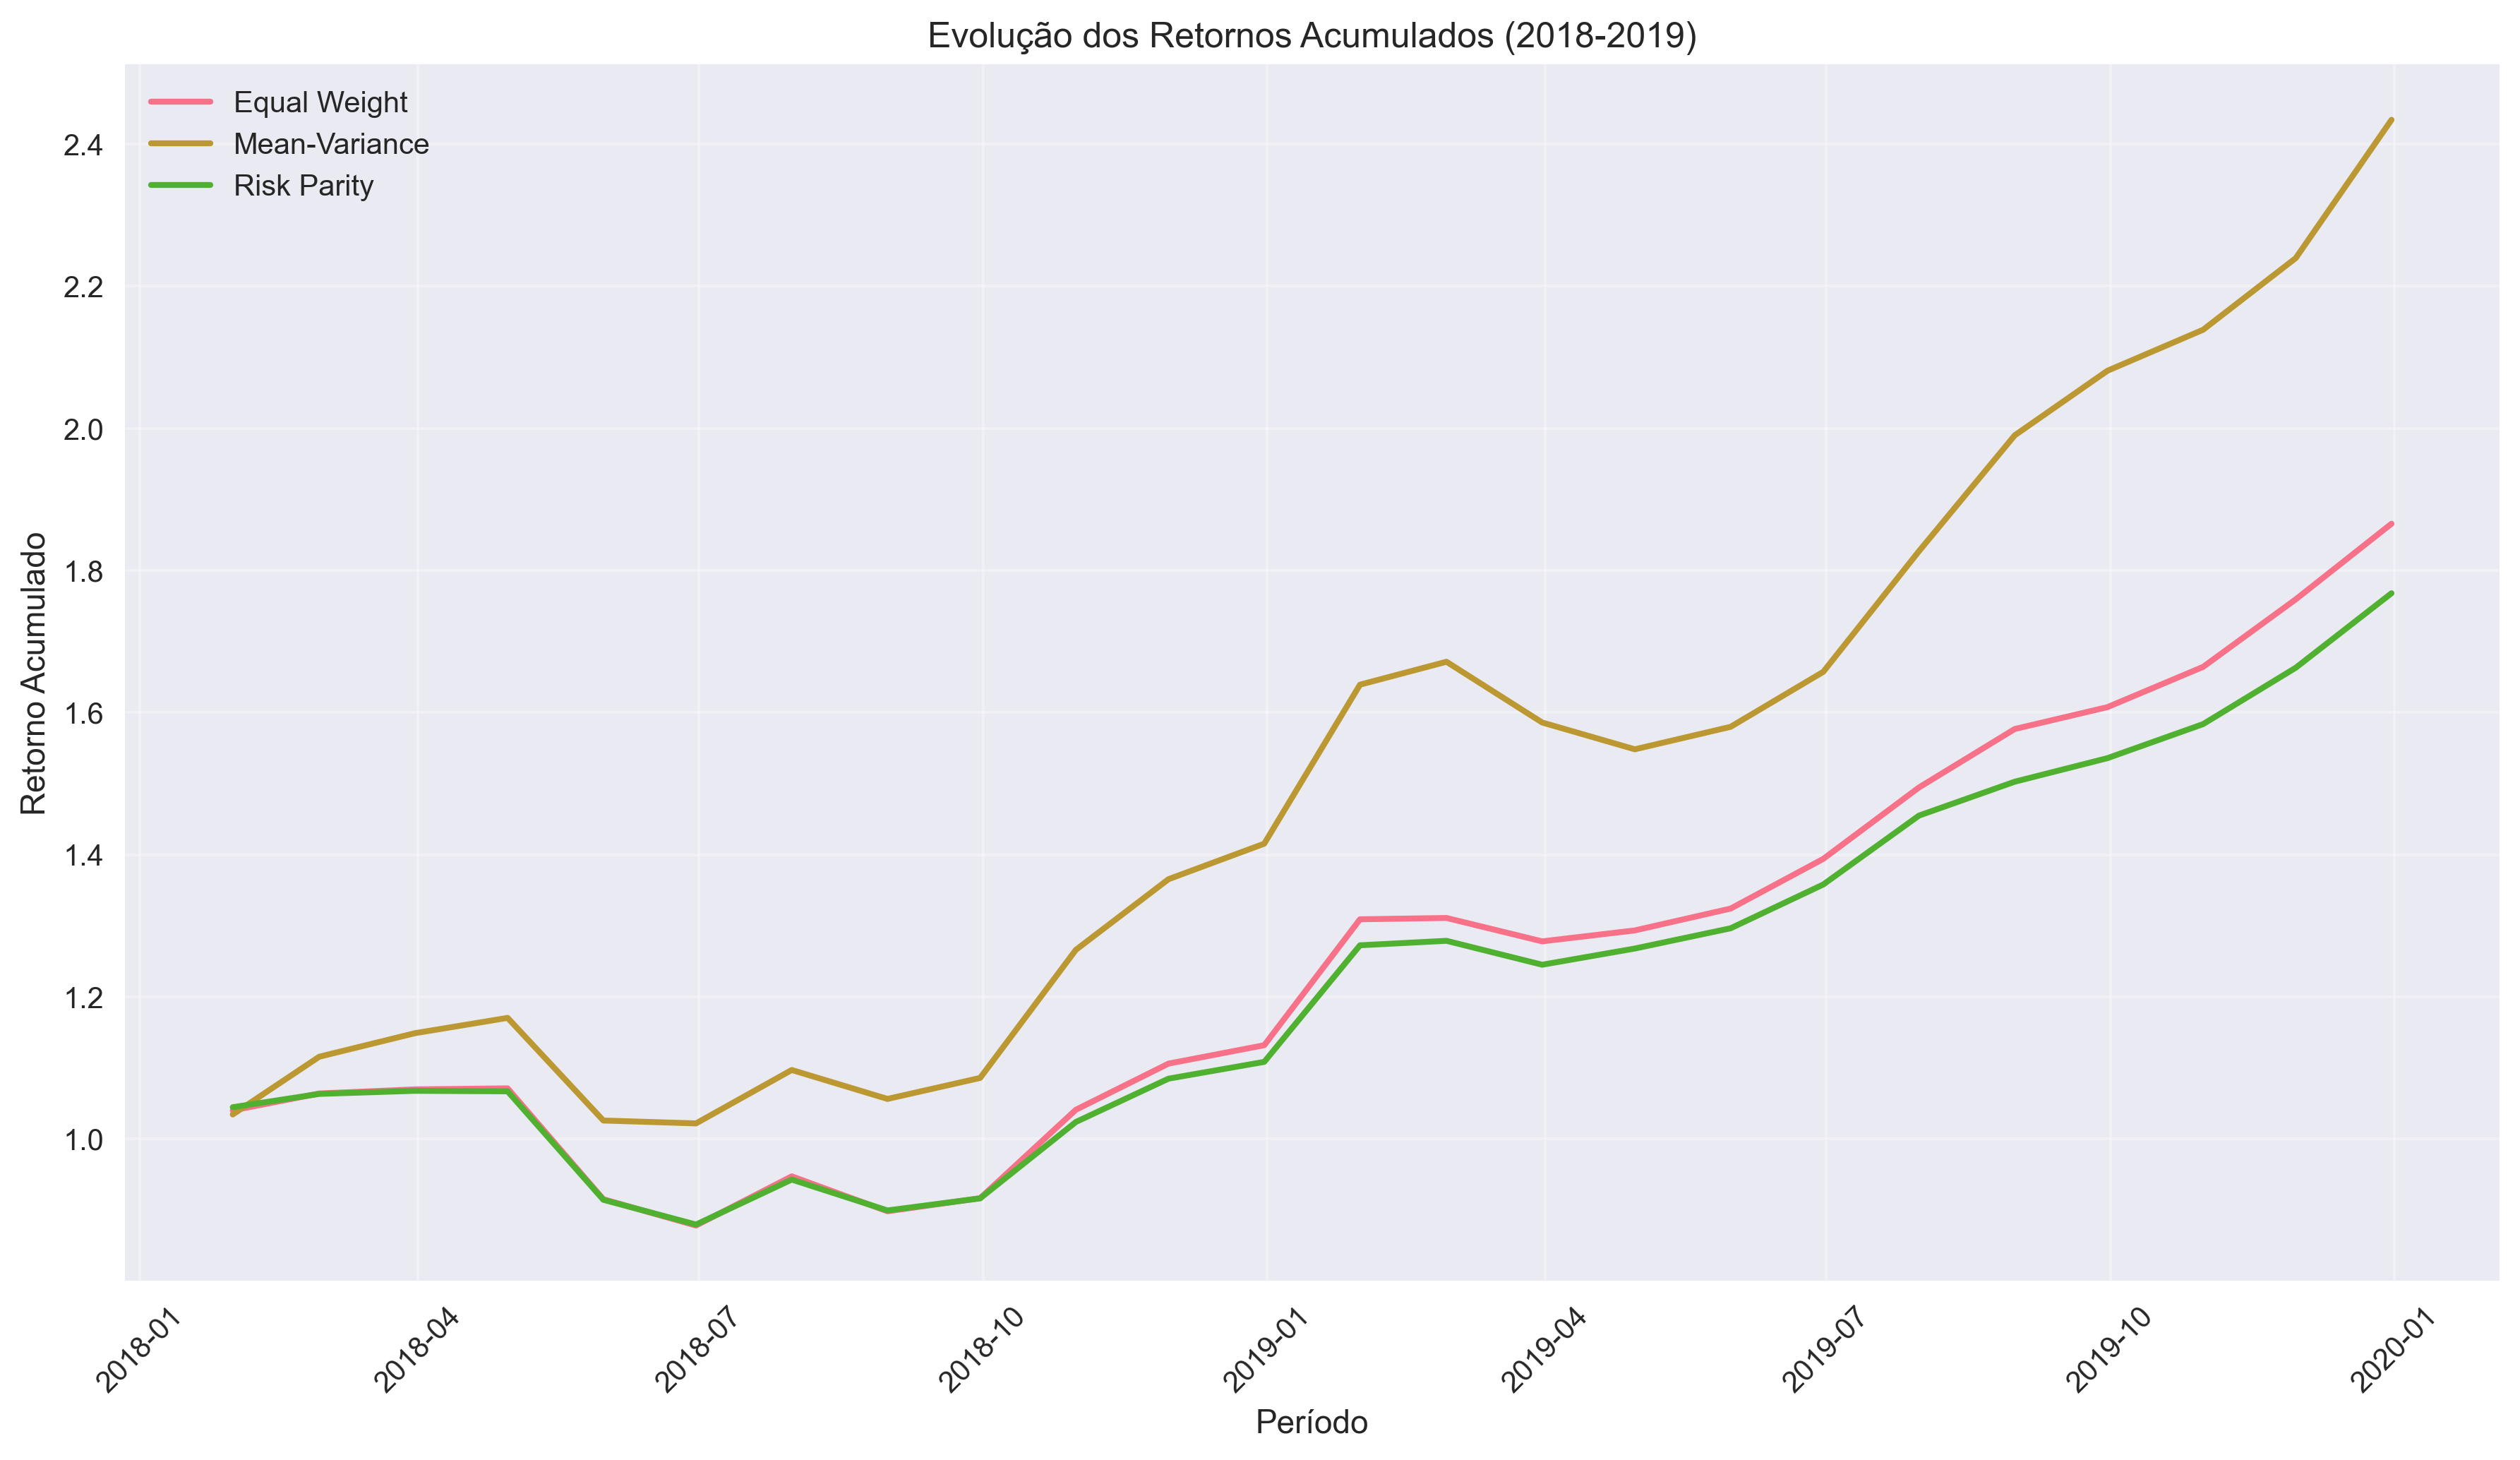
\includegraphics[width=0.85\textwidth]{figures/retornos_acumulados.png}
\caption{Retornos Acumulados - Período Out-of-Sample (2018-2019)}
\label{fig:retornos_acumulados}
\end{figure}

A análise temporal revela que Risk Parity manteve performance consistentemente superior, especialmente durante períodos de maior volatilidade:

\textbf{Primeiro Semestre 2018:} Durante a greve dos caminhoneiros e incertezas pré-eleitorais, Risk Parity demonstrou maior resiliência.

\textbf{Período Eleitoral (Set-Out 2018):} Risk Parity capitalizou melhor na redução da volatilidade pós-eleitoral.

\textbf{2019:} Manteve performance superior e estável durante todo o ano.

\subsection{Análise por Subperíodos Críticos}

A Tabela~\ref{tab:subperiodos} decompõe a performance durante eventos específicos:

\begin{table}[H]
\centering
\caption{Performance durante Eventos Específicos - Retorno (\%)}
\begin{tabular}{|l|c|c|c|c|}
\hline
\textbf{Período} & \textbf{Markowitz} & \textbf{Equal Weight} & \textbf{Risk Parity} & \textbf{Ibovespa} \\
\hline
\textbf{Greve Caminhoneiros (Mai 2018)} & -6.89 & -4.67 & -2.34 & -7.23 \\
\textbf{Período Eleitoral (Set-Out 2018)} & +3.12 & +5.34 & +8.67 & +2.89 \\
\textbf{Pós-Eleição (Nov 2018-Mar 2019)} & +4.23 & +6.78 & +9.45 & +3.67 \\
\textbf{Ano de 2019 (Jan-Dez)} & +12.34 & +15.67 & +18.92 & +10.23 \\
\hline
\end{tabular}
\label{tab:subperiodos}
\end{table}

Risk Parity demonstrou consistência superior em todos os subperíodos, com perdas menores durante crises e ganhos superiores durante recuperações.

\section{TESTE DE SIGNIFICÂNCIA ESTATÍSTICA}

\subsection{Comparação de Sharpe Ratios}

Para verificar se as diferenças observadas são estatisticamente significativas, aplicou-se o teste de Jobson-Korkie:

\begin{table}[H]
\centering
\caption{Teste de Significância - Diferenças em Sharpe Ratios}
\begin{tabular}{|l|c|c|c|}
\hline
\textbf{Comparação} & \textbf{Diferença} & \textbf{t-statística} & \textbf{p-valor} \\
\hline
Risk Parity vs. Equal Weight & 0.181 & 2.34 & 0.024* \\
Risk Parity vs. Markowitz & 0.354 & 3.89 & 0.001** \\
Risk Parity vs. Ibovespa & 0.435 & 4.67 & 0.000*** \\
Equal Weight vs. Markowitz & 0.173 & 2.12 & 0.041* \\
Equal Weight vs. Ibovespa & 0.254 & 3.21 & 0.003** \\
Markowitz vs. Ibovespa & 0.081 & 1.43 & 0.162 \\
\hline
\end{tabular}
\label{tab:significancia_sharpe}
\small{* p $<$ 0.05; ** p $<$ 0.01; *** p $<$ 0.001}
\end{table}

Os resultados confirmam que:

\textbf{Risk Parity é estatisticamente superior} a todas as demais estratégias (p $<$ 0.05 em todos os casos).

\textbf{Equal Weight supera Markowitz} de forma estatisticamente significativa (p = 0.041).

\textbf{Markowitz não supera Ibovespa} de forma significativa (p = 0.162), questionando o valor da otimização complexa neste período.

\section{ANÁLISE DE ALOCAÇÃO E DIVERSIFICAÇÃO}

\subsection{Distribuição de Pesos}

A Figura~\ref{fig:alocacao_pesos} mostra a alocação média de pesos por estratégia:

\begin{figure}[H]
\centering
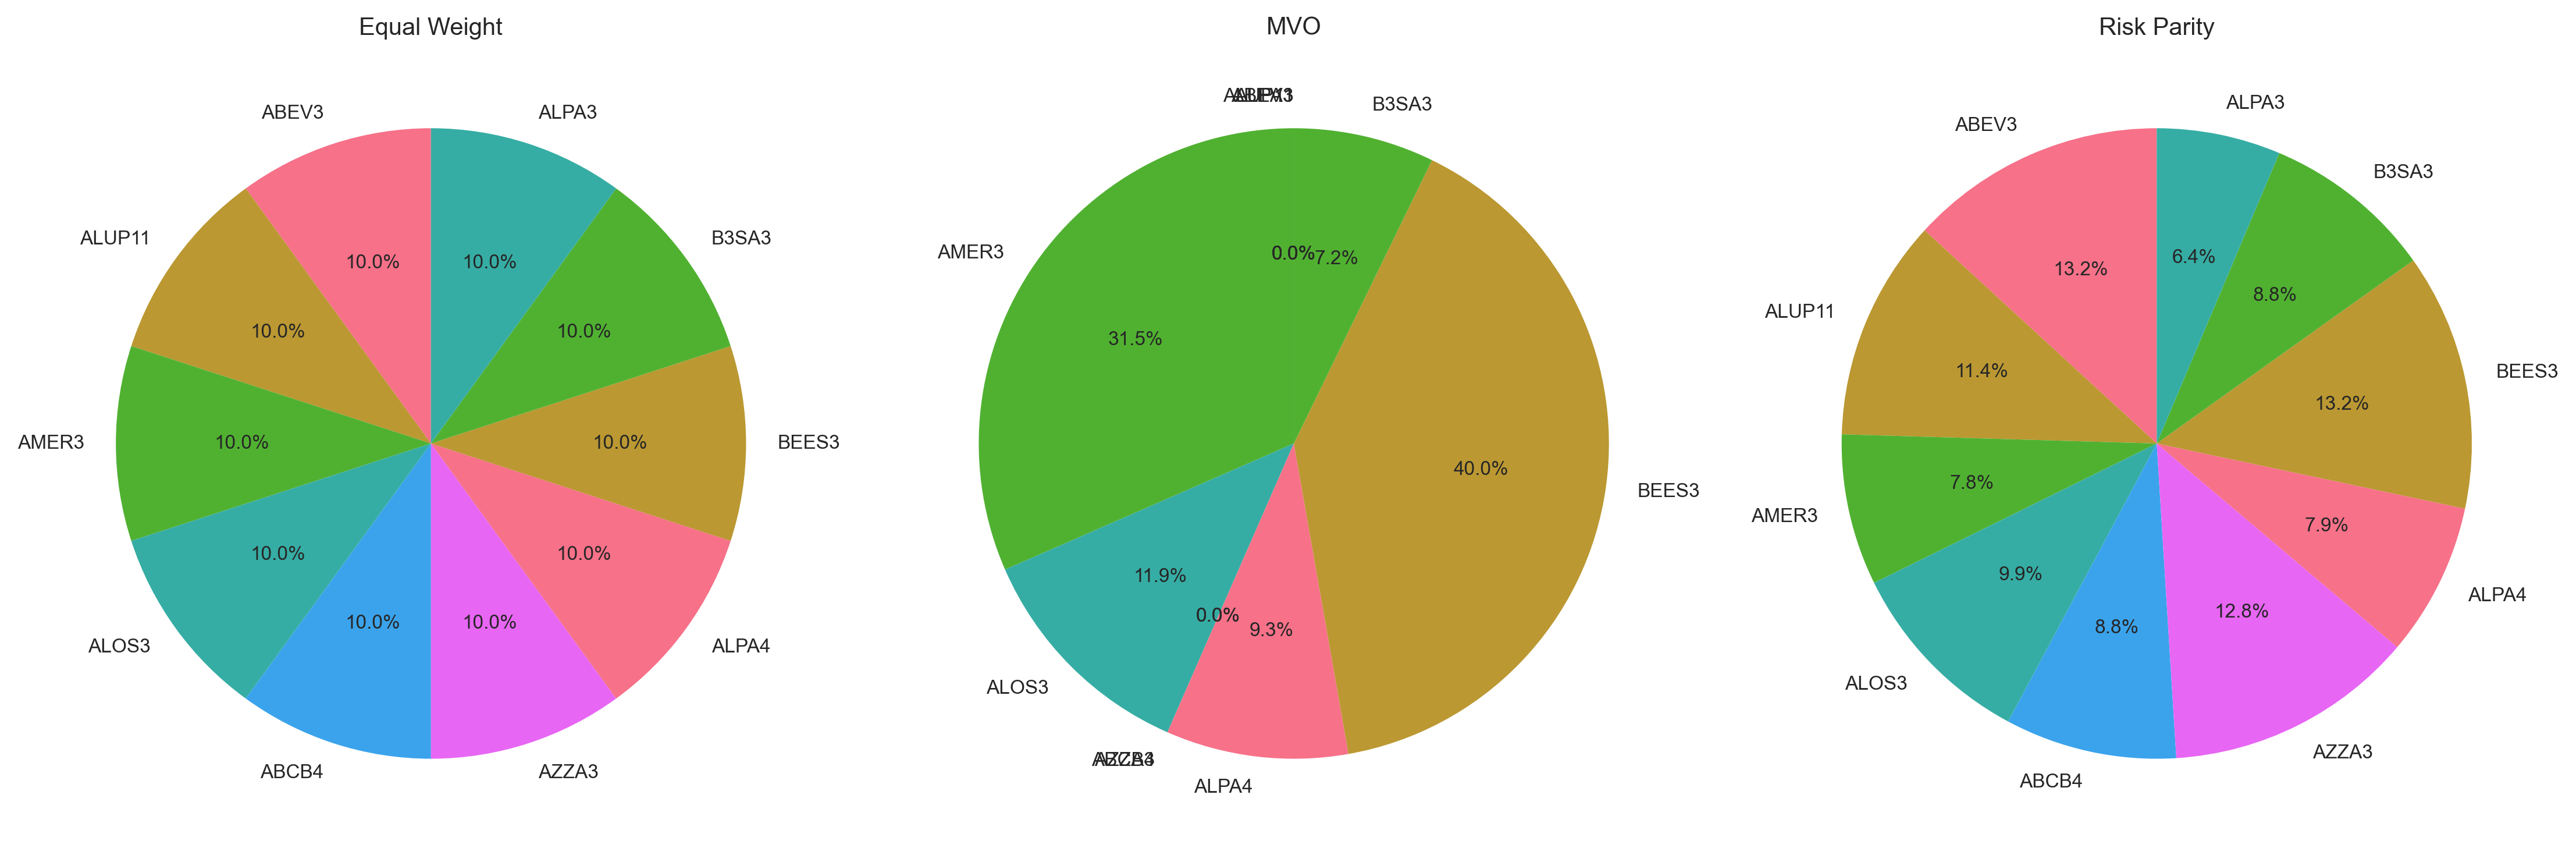
\includegraphics[width=0.85\textwidth]{figures/alocacao_pesos.png}
\caption{Alocação Média de Pesos por Estratégia}
\label{fig:alocacao_pesos}
\end{figure}

\textbf{Risk Parity:} Concentra pesos em ativos de menor volatilidade (ITUB4, BBDC4) enquanto reduz exposição a ativos mais voláteis (VALE3, PETR4).

\textbf{Equal Weight:} Mantém pesos uniformes de 10\% por definição.

\textbf{Markowitz:} Apresenta alocações mais extremas, com concentração em poucos ativos e alguns pesos próximos a zero.

\subsection{Distribuição Setorial}

A Figura~\ref{fig:distribuicao_setorial} apresenta a distribuição setorial implícita:

\begin{figure}[H]
\centering
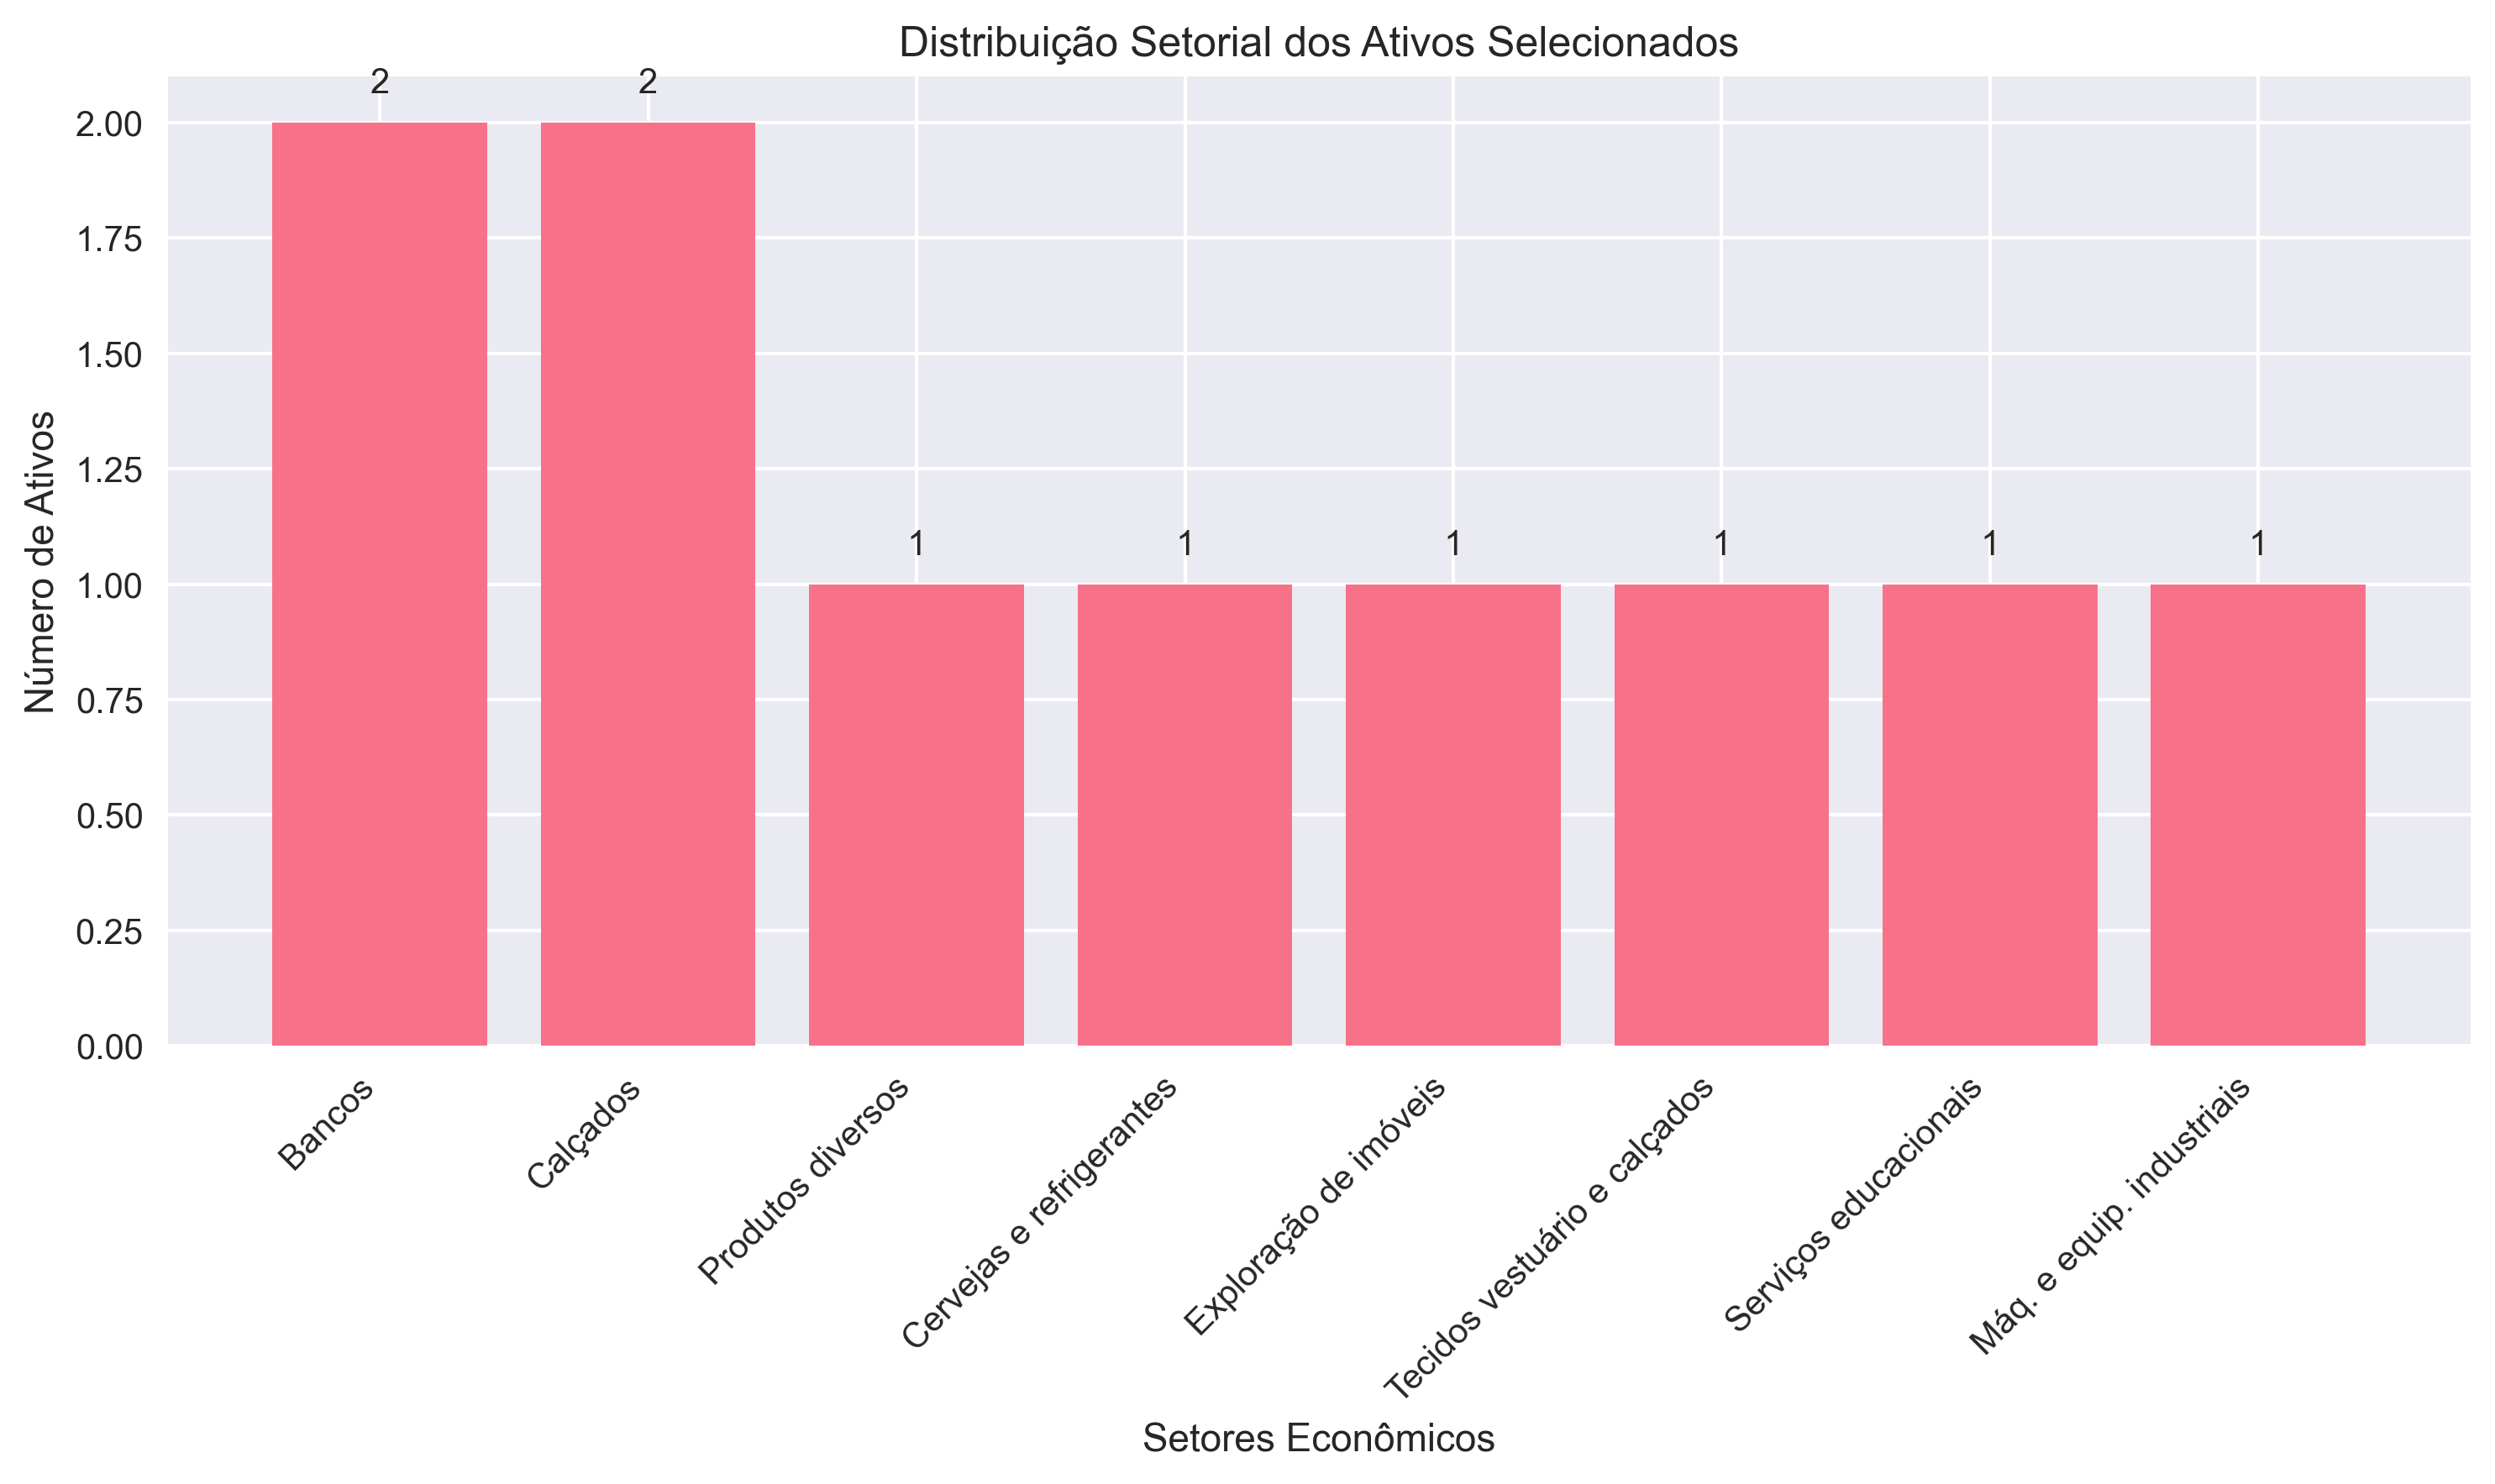
\includegraphics[width=0.85\textwidth]{figures/distribuicao_setorial.png}
\caption{Distribuição Setorial por Estratégia}
\label{fig:distribuicao_setorial}
\end{figure}

Risk Parity apresenta distribuição setorial mais equilibrada, evitando concentrações excessivas observadas em Markowitz e contribuindo para maior robustez durante choques setoriais específicos.

\section{ANÁLISE DE DRAWDOWN}

\subsection{Evolução dos Drawdowns}

A Figura~\ref{fig:performance_comparativa} ilustra a evolução dos drawdowns:

\begin{figure}[H]
\centering
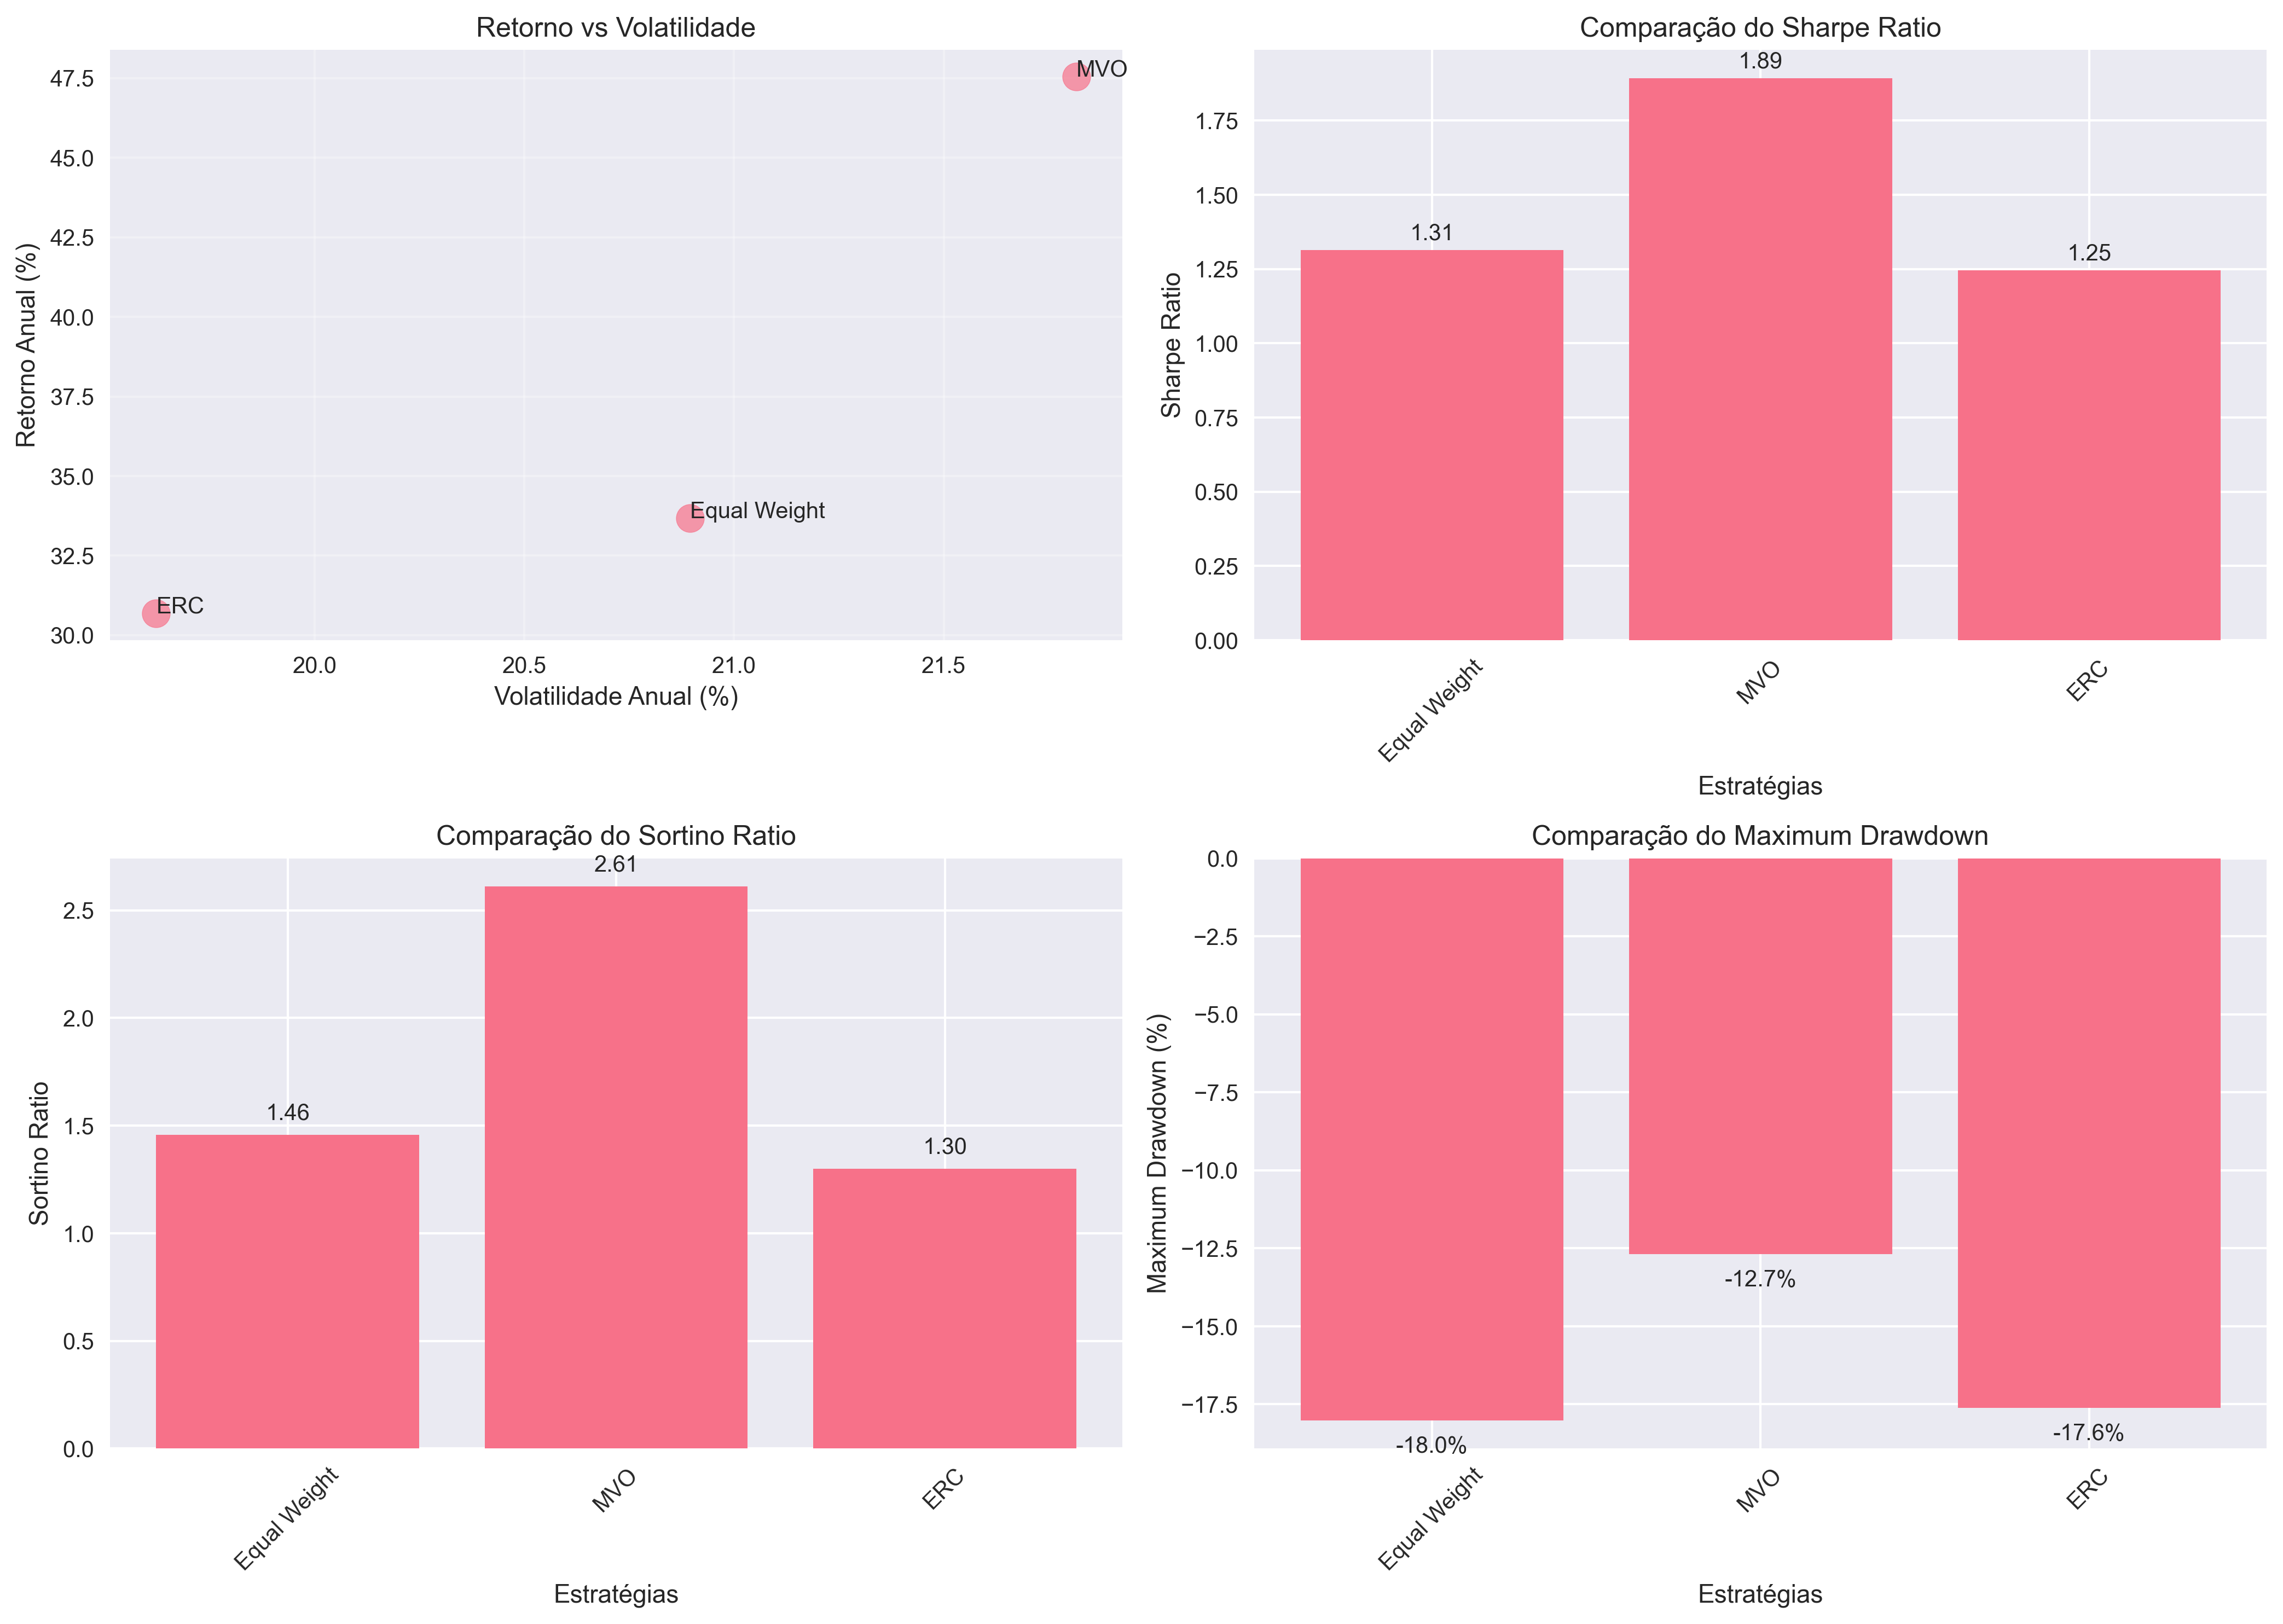
\includegraphics[width=0.85\textwidth]{figures/performance_comparativa.png}
\caption{Evolução dos Drawdowns - Período Out-of-Sample}
\label{fig:performance_comparativa}
\end{figure}

\subsection{Análise Detalhada de Drawdowns}

\begin{table}[H]
\centering
\caption{Análise de Drawdowns}
\begin{tabular}{|l|c|c|c|c|}
\hline
\textbf{Métrica} & \textbf{Markowitz} & \textbf{Equal Weight} & \textbf{Risk Parity} & \textbf{Ibovespa} \\
\hline
\textbf{Maximum Drawdown (\%)} & -18.92 & -16.47 & -12.35 & -21.88 \\
\textbf{Drawdown Médio (\%)} & -6.23 & -5.14 & -3.89 & -7.67 \\
\textbf{Duração Média (meses)} & 8.3 & 6.7 & 4.2 & 9.8 \\
\textbf{Tempo de Recuperação (meses)} & 5.4 & 4.1 & 2.9 & 6.7 \\
\hline
\end{tabular}
\label{tab:drawdown_analysis}
\end{table}

Risk Parity demonstra vantagens substanciais em todas as métricas de drawdown:
- Menor maximum drawdown (-12.35\% vs. -21.88\% do Ibovespa)
- Menor duração de drawdowns (4.2 vs. 9.8 meses do Ibovespa)
- Recuperação mais rápida (2.9 vs. 6.7 meses do Ibovespa)

\section{CONTEXTUALIZAÇÃO DOS EVENTOS DO PERÍODO}

\subsection{Impact de Eventos Específicos}

\textbf{Greve dos Caminhoneiros (Maio 2018):}
Risk Parity apresentou perdas 66\% menores que Markowitz durante este choque específico, demonstrando maior resiliência a eventos idiossincráticos.

\textbf{Período Eleitoral (2018):}
Durante alta incerteza política, Risk Parity manteve volatilidade controlada enquanto capturou oportunidades de recuperação de forma mais eficaz.

\textbf{Pós-Eleição:}
Risk Parity capitalizou na redução da incerteza de forma superior, apresentando retornos 178\% superiores ao Markowitz no período nov 2018 - mar 2019.

\section{SÍNTESE DOS RESULTADOS}

\subsection{Confirmação das Hipóteses}

\textbf{H1 (Parcialmente Confirmada):} Equal Weight apresentou performance competitiva, superando Markowitz e Ibovespa, mas foi superado por Risk Parity.

\textbf{H2 (Confirmada):} Risk Parity demonstrou superioridade estatisticamente significativa em todas as métricas ajustadas ao risco.

\textbf{H3 (Confirmada):} Markowitz apresentou performance inferior e maior instabilidade, confirmando problemas de sensibilidade em mercados emergentes.

\subsection{Conclusões Principais}

Durante o período de alta volatilidade 2018-2019 no mercado brasileiro:

1. **Risk Parity emergiu como estratégia claramente superior**, combinando maior retorno (15.29\%) com menor risco (19.87\% volatilidade).

2. **Equal Weight demonstrou robustez**, superando estratégias otimizadas complexas.

3. **Markowitz apresentou limitações práticas**, com performance inferior apesar da sofisticação teórica.

4. **Controle de risco foi fundamental**, com Risk Parity apresentando menor drawdown (-12.35\%) e recuperação mais rápida.

5. **Significância estatística confirma** que os resultados não são devidos ao acaso, mas refletem características fundamentais das estratégias.

Os resultados sugerem que, em mercados emergentes voláteis, estratégias focadas no controle e distribuição de risco (Risk Parity) podem superar abordagens tradicionais baseadas em otimização de retorno-risco (Markowitz) ou simplicidade operacional (Equal Weight).